\chapter{آنچه باید بدانید}\label{App:App1}
در این بخش با نحوه مناسب درج منابع، نمونه مثال‌هایی از جدول، نمودار و الگوریتم در لاتک  آشنا خواهیم شد.



\section{ مدیریت مراجع با \texorpdfstring{\lr{Bib\TeX}}{Bib\TeX} }
در بخش \ref{Sec:Ref} اشاره شد که با دستور  \lr{\textbackslash bibitem}
  می‌توان یک مرجع را تعریف نمود و با فرمان \lr{\textbackslash cite}
  به آن ارجاع داد. این روش برای تعداد مراجع زیاد و تغییرات آن‌ها مناسب نیست. در ادامه به صورت مختصر توضیحی در خصوص برنامه \lr{BibTeX} که همراه با توزیع‌های معروف تِک عرضه می‌شود و نحوه استفاده از آن در زی‌پرشین خواهیم داشت.
  
یکی از روش‌های قدرتمند و انعطاف‌پذیر برای نوشتن مراجع مقالات و مدیریت مراجع در لاتک، استفاده از  \lr{BibTeX} 
 است.  روش کار با  \lr{BibTeX} به‌این صورت است که مجموعهٔ همه‌ٔ مراجعی را که در پایان‌نامه/رساله استفاده کرده یا خواهیم کرد، 
در پروندهٔ جداگانه‌ای نوشته و به آن فایل در سند خودمان به صورت مناسب لینک می‌دهیم.
 کنفرانس‌ها یا مجله‌های گوناگون برای نوشتن مراجع، قالب‌ها یا قراردادهای متفاوتی دارند که به آن‌ها استایلهای مراجع گفته می‌شود.
 در این حالت به کمک ‌استایل‌های \lr{BibTeX} خواهید توانست تنها با تغییر یک پارامتر در پروندهٔ ورودی خود، مراجع را مطابق قالب موردنظر تنظیم کنید. 
 بیشتر مجلات و کنفرانس‌های معتبر یک پروندهٔ سبک (\lr{BibTeX Style}) با پسوند \lr{bst} در وب‌گاه خود می‌گذارند که برای همین منظور طراحی شده است.

به جز نوشتن مقالات این سبک‌ها کمک بسیار خوبی برای تهیهٔ مستندات علمی همچون پایان‌نامه‌هاست که فرد می‌تواند هر قسمت از کارش را که نوشت مراجع مربوطه را به بانک مراجع خود اضافه نماید. با داشتن چنین بانکی از مراجع، وی خواهد توانست به راحتی یک یا چند ارجاع به مراجع و یا یک یا چند بخش را حذف یا اضافه ‌نماید؛ 
مراجع به صورت خودکار مرتب شده و فقط مراجع ارجاع داده شده در قسمت کتاب‌نامه خواهندآمد. قالب مراجع به صورت یکدست مطابق سبک داده شده بوده و نیازی نیست که کاربر درگیر قالب‌دهی به مراجع باشد. 

در حال حاضر چندین قالب (استایل یا سبک) فارسی قابل استفاده هستند که توسط دکتر محمود امین‌طوسی آماده شده‌اند و در توزیع‌های تک‌لایو 
و میک‌تک موجود می‌باشند. 

با استفاده از استایل فوق می‌توانید به انواع مختلفی از مراجع فارسی و لاتین ارجاع دهید. به عنوان نمونه مرجع 
\cite{Omidali82phdThesis}
 یک نمونه پروژه دکترا (به فارسی) و مرجع 
\cite{Vahedi87} یک نمونه مقاله مجله فارسی است.
مرجع 
\cite{Amintoosi87afzayesh}  یک نمونه  مقاله کنفرانس فارسی و
مرجع 
\cite{Pedram80osool} یک نمونه کتاب فارسی با ذکر مترجمان و ویراستاران فارسی است. مرجع 
\cite{Khalighi07MscThesis} یک نمونه پروژه کارشناسی ارشد انگلیسی و
\cite{xepersian} هم یک نمونه متفرقه  می‌باشند.

مراجع 
\cite{Gonzalez02book,Baker02limits} 
نمونه کتاب و مقاله انگلیسی هستند.


\subsection{ نحوه استفاده از سبک‌های فارسی}


برای استفاده از بیب‌تک باید مراجع خود را در یک فایل با پسوند \lr{bib} ذخیره نمایید. یک فایل \lr{bib} در واقع یک پایگاه داده از مراجع\LTRfootnote{Bibliography Database}  شماست که هر مرجع در آن به عنوان یک رکورد از این پایگاه داده
با قالبی خاص ذخیره می‌شود. به هر رکورد یک مدخل\LTRfootnote{Entry} گفته می‌شود. یک نمونه مدخل برای معرفی کتاب \lr{Digital Image Processing} در ادامه آمده است:

\begin{Verbatim}
@BOOK{Gonzalez02image,
  AUTHOR =      {Rafael Gonzalez and Richard Woods},
  TITLE =       {Digital Image Processing},
  PUBLISHER =   {Prentice-Hall, Inc.},
  YEAR =        {2006},
  EDITION =     {3rd},
  ADDRESS =     {Upper Saddle River, NJ, USA}
}
\end{Verbatim}

در مثال فوق، \lr{@BOOK} مشخصهٔ شروع یک مدخل مربوط به یک کتاب و \lr{Gonzalez02book} برچسبی است که به‌این مرجع منتسب شده است.
 این برچسب بایستی یکتا باشد. برای آنکه فرد به راحتی بتواند برچسب مراجع خود را به خاطر بسپارد و حتی‌الامکان برچسب‌ها متفاوت با هم باشند معمولاً از قوانین خاصی به‌این منظور استفاده می‌شود. یک قانون می‌تواند فامیل نویسندهٔ اول+دو رقم سال نشر+اولین کلمهٔ عنوان اثر باشد. به \lr{AUTHOR} و $\dots$ و \lr{ADDRESS} فیلدهای این مدخل گفته می‌شود؛ که هر یک با مقادیر مربوط به مرجع مقدار گرفته‌اند. ترتیب فیلدها مهم نیست. 

انواع متنوعی از مدخل‌ها برای اقسام مختلف مراجع همچون کتاب، مقالهٔ کنفرانس و مقالهٔ ژورنال وجود دارد که برخی فیلدهای آن‌ها با هم متفاوت است. 
نام فیلدها بیانگر نوع اطلاعات آن می‌باشد. مثال‌های ذکر شده در فایل \lr{references.bib} کمک خوبی به شما خواهد بود. 
با استفاده از سبک‌های فارسی آماده شده، محتویات هر فیلد می‌تواند به فارسی نوشته شود، ترتیب مراجع و نحوهٔ چینش فیلدهای هر مرجع را سبک مورد استفاده  مشخص خواهد کرد.

برای عمل به‌این روش: 
\textbf{در فایل \lr{references.bib}
 که همراه با این پایان‌نامه/رساله هست، موارد مختلفی درج شده است، کافیست مراجع خود را جایگزین موارد مندرج در آن نمایید.}

پس از قرار دادن مراجع خود، یک بار \lr{XeLaTeX} را روی سند خود اجرا نمایید، سپس \lr{bibtex} و پس از آن دوبار \lr{XeLaTeX} را. 
در 
\lr{TeXstudio} و
\lr{TeXMaker} کلید \lr{F11} و در \lr{TeXWorks} هم گزینهٔ \lr{BibTeX} از منوی \lr{Typeset}، \lr{BibTeX} را روی سند شما اجرا می‌کنند.

برای بسیاری از مقالات لاتین حتی لازم نیست که مدخل مربوط به آنرا خودتان بنویسید. با جستجوی نام مقاله + کلمه \lr{bibtex}  در اینترنت سایتهای بسیاری همچون \lr{ACM} و \lr{ScienceDirect} را خواهید یافت که مدخل \lr{bibtex} مربوط به مقاله شما را دارند و کافیست آنرا به انتهای فایل \lr{MyReferences} اضافه کنید.

%از هر یک از سبکهای \lr{Persian-bib} می‌توانید استفاده کنید، البته اگر از سه استایل آخر استفاده می‌کنید و مایلید که مراجع شما شماره بخورند باید بسته \lr{natbib} را با گزینه \lr{numbers} فراخوانی نمایید.

\section{جدول}
رسم جدول نیز در لاتک کار سختی نیست.  جدول 
\eqref{tab:MotionModels}
مدل‌های تبدیل را نشان می‌دهد.

\begin{table}[ht]
\caption{مدلهای تبدیل.}
\label{tab:MotionModels}
\centering
\onehalfspacing
\begin{tabular}{|r|c|l|r|}
\hline نام مدل & درجه آزادی & تبدیل مختصات & توضیح \\ 
\hline انتقالی & ۲ & $\begin{aligned} x'=x+t_x \\ y'=y+t_y \end{aligned}$  &  انتقال دوبعدی\\ 
\hline اقلیدسی & ۳ & $\begin{aligned} x'=xcos\theta - ysin\theta+t_x \\ y'=xsin\theta+ycos\theta+t_y \end{aligned}$  &  انتقالی+دوران \\ 
\hline 
\end{tabular} 
\end{table}




\section{درج الگوریتم}
\subsection{الگوریتم با دستورات فارسی}
 الگوریتم 
 \eqref{alg:DLT} 
 یک الگوریتم با دستورات فارسی است.
\begin{algorithm}[t]
\onehalfspacing
\caption{الگوریتم \lr{DLT} برای تخمین ماتریس هوموگرافی.} \label{alg:DLT}
\begin{algorithmic}[1]
\REQUIRE $n\geq4$ زوج نقطهٔ متناظر در دو تصویر 
${\mathbf{x}_i\leftrightarrow\mathbf{x}'_i}$،\\
\ENSURE ماتریس هوموگرافی $H$ به نحوی‌که: 
$\mathbf{x}'_i = H \mathbf{x}_i$.
  \STATE برای هر زوج نقطهٔ متناظر
$\mathbf{x}_i\leftrightarrow\mathbf{x}'_i$ 
ماتریس $\mathbf{A}_i$ را با استفاده از رابطهٔ \ref{eq:DLT_Ah} محاسبه کنید.
  \STATE ماتریس‌های ۹ ستونی  $\mathbf{A}_i$ را در قالب یک ماتریس $\mathbf{A}$ ۹ ستونی ترکیب کنید. 
  \STATE تجزیهٔ مقادیر منفرد \lr{(SVD)}  ماتریس $\mathbf{A}$ را بدست آورید. بردار واحد متناظر با کمترین مقدار منفرد جواب $\mathbf{h}$ خواهد بود.
  \STATE  ماتریس هوموگرافی $H$ با تغییر شکل $\mathbf{h}$ حاصل خواهد شد.
\end{algorithmic}
\end{algorithm}

\subsection{الگوریتم با دستورات لاتین}
الگوریتم
 \ref{alg:RANSAC}
  یک الگوریتم با دستورات لاتین است.

\begin{algorithm}[t]
\onehalfspacing
\caption{الگوریتم \lr{RANSAC} برای تخمین ماتریس هوموگرافی.} \label{alg:RANSAC}
\begin{latin}
\begin{algorithmic}[1]
\REQUIRE $n\geq4$ putative correspondences, number of estimations, $N$, distance threshold $T_{dist}$.\\
\ENSURE Set of inliers and Homography matrix $H$.
\FOR{$k = 1$ to $N$}
  \STATE Randomly choose 4 correspondence,
  \STATE Check whether these points are colinear, if so, redo the above step
  \STATE Compute the homography $H_{curr}$ by DLT algorithm from the 4 points pairs,
  \STATE $\ldots$ % الگوریتم کامل نیست
  \ENDFOR
  \STATE Refinement: re-estimate H from all the inliers using the DLT algorithm.
\end{algorithmic}
\end{latin}
\end{algorithm}


\section{درج کد}
درج کد به زبانهای مختلف نیز به سادگی امکان‌پذیر است. برنامه 
\ref{Code:MATLAB1}
یک قطعه کد \lr{MATLAB} را نشان می‌دهد.
%\begin{figure}
%\begin{latin}
\begin{lstlisting}[language=MATLAB,breaklines=true,numbers=right, numberstyle=\footnotesize, numbersep=-10pt,  frame=single, breakatwhitespace=false,
caption={نمونه کد \lr{MATLAB}},label={Code:MATLAB1}]
% define a continuous function
f = '4*sin(2*pi*t)';
ezplot(f);
for i=1:10
    disp(i)
end
\end{lstlisting}
%\end{latin}


%\end{figure}
%\doublespacing


\section{فرمول‌های ریاضی}
تقریباً هر آنچه دانشجویان برای نوشتن فرمول‌های ریاضی لازم دارند، در کتاب 
\lr{mathmode}
آمده است. کافیست در خط فرمان دستور زیر را وارد کنید:
\begin{latin}
texdoc mathmode
\end{latin}
متن زیر یک متن شامل انواعی از اشیاء ریاضی است که با ملاحظه فایل \lr{.tex} این سند می‌توانید دستورات مربوطه را مشاهده فرمایید.

شناخته‌شده‌ترین روش تخمین ماتریس هوموگرافی الگوریتم تبدیل خطی مستقیم 
%(\lr{DLT\LTRfootnote{Direct Linear Transform}}) 
است.  فرض کنید چهار زوج نقطهٔ متناظر در دو تصویر در دست هستند،  $\mathbf{x}_i\leftrightarrow\mathbf{x}'_i$   و تبدیل با رابطهٔ
  $\mathbf{x}'_i = H\mathbf{x}_i$
  نشان داده می‌شود که در آن:
\[\mathbf{x}'_i=(x'_i,y'_i,w'_i)^\top  \]
و $H$ ماتریس تبدیل است.
رابطه زیر را برای الگوریتم  \eqref{alg:DLT} لازم دارم.
\begin{equation}\label{eq:DLT_Ah}
\left[
\begin{array}{ccc}
0^\top & -w'_i\mathbf{x}_i^\top & y'_i\mathbf{x}_i^\top \\ 
w'_i\mathbf{x}_i & 0^\top & -x'_i\mathbf{x}_i^\top \\ 
- y'_i\mathbf{x}_i^\top & x'_i\mathbf{x}_i^\top & 0^\top
\end{array} 
\right]
\left(
\begin{array}{c}
\mathbf{h}^1 \\ 
\mathbf{h}^2 \\ 
\mathbf{h}^3
\end{array} 
\right)=0
\end{equation}

\section{نمودار}

لاتک بسته‌هایی با قابلیت‌های زیاد برای رسم انواع مختلف نمودارها دارد. مانند بسته‌های \lr{Tikz} و  \lr{PSTricks}. 
توضیح اینها فراتر از این پیوست کوچک است.%
\footnote{
نمونه مثال‌هایی از بسته \lr{Tikz} را می‌توانید
 در \url{http://www.texample.net/tikz/examples/} ببینید. به دانشجویانی که قصد قرار دادن اشکالی همانند گراف در سند خود را دارند، توصیه می‌شود مثال‌هایی از سایت مذکور را ملاحظه فرمایند.}
یک نمونه نمودار رسم شده با بستهٔ 
\lr{TikZ}
 در شکل 
\ref{fig:parabola}
نشان داده شده است.
\begin{figure}[t]
\centering
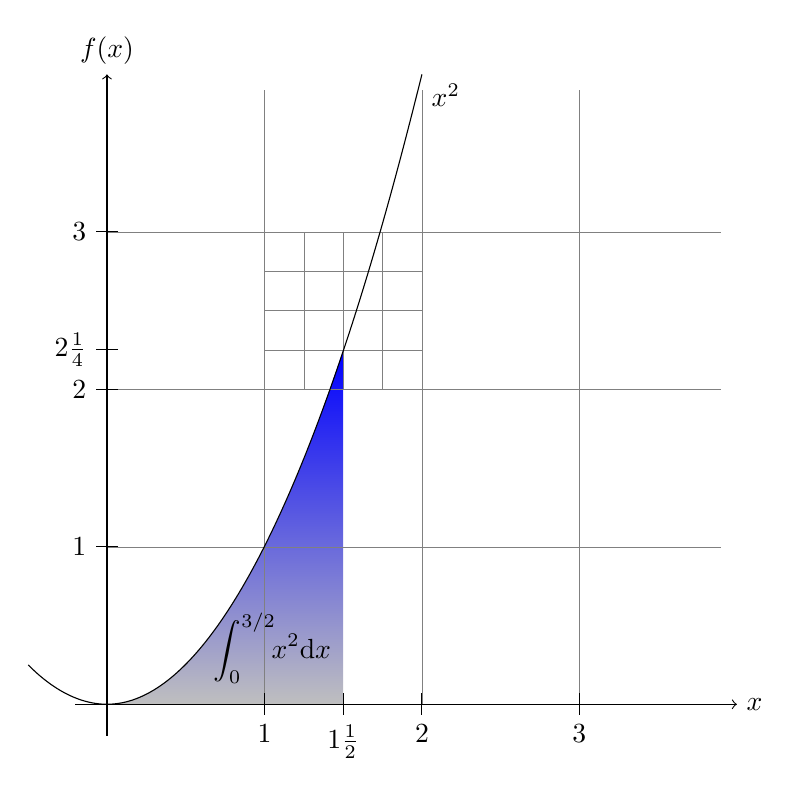
\begin{tikzpicture}[scale=2]
  \shade[top color=blue,bottom color=gray!50] 
      (0,0) parabola (1.5,2.25) |- (0,0);
  \draw (1.05cm,2pt) node[above] 
      {$\displaystyle\int_0^{3/2} \!\!x^2\mathrm{d}x$};

  \draw[style=help lines] (0,0) grid (3.9,3.9)
       [step=0.25cm]      (1,2) grid +(1,1);

  \draw[->] (-0.2,0) -- (4,0) node[right] {$x$};
  \draw[->] (0,-0.2) -- (0,4) node[above] {$f(x)$};

  \foreach \x/\xtext in {1/1, 1.5/1\frac{1}{2}, 2/2, 3/3}
    \draw[shift={(\x,0)}] (0pt,2pt) -- (0pt,-2pt) node[below] {$\xtext$};

  \foreach \y/\ytext in {1/1, 2/2, 2.25/2\frac{1}{4}, 3/3}
    \draw[shift={(0,\y)}] (2pt,0pt) -- (-2pt,0pt) node[left] {$\ytext$};

  \draw (-.5,.25) parabola bend (0,0) (2,4) node[below right] {$x^2$};
\end{tikzpicture}
\caption{یک نمودار زیبا با ارقام فارسی و قابلیت بزرگ‌نمایی بسیار، بدون از دست دادن کیفیت.}
\label{fig:parabola}
\end{figure}
موقعیت قرارگیری اشیاء شناور مانند جدول و تصویر توسط خود لاتک مدیریت می‌شود. 
گاهی موقعیت مناسب پیدا نمی‌شود و این موارد در بافر قرار می‌گیرند و در انتهای بخش یا فصل نمایش داده می‌شوند. 
برای ملزم کردن لاتک به نمایش اشیايی که در بافر دارد کافیست از دستور 
\verb!\clearpage!
استفاده کنیم.

 گاهی  ممکن است لازم باشد خودمان دستور رفتن به صفحه جدید را با دستور 
\verb!\newpage!
به لاتک بدهیم، مثل الان ...
\newpage




\section{درج توضیحات در حاشیه}
\setLTRparagraphfootnotes
فراگیر شدن اینترنت ارتباطات از راه دور را سهل نموده است. فرض کنید دانشجو \linebreak 
پایان‌نامه/رساله خود را نوشته و از طریق اینترنت برای اظهار نظر به استاد راهنمای خود رسانده است. 
اگر قرار باشد استاد راهنما پس از مطالعه پایان‌نامه/رساله، مواردی را  گوشزد نماید، به جز راه‌های معمول (تلفن و ایمیل و ...) یک راهکار مناسب استفاده از بسته 
\lr{todonotes}
در لاتک است. به کمک این بسته که جناب آقای خلیقی از نسخه ۱۶ بسته
\lr{bidi}
امکان استفاده از آن‌را برای فارسی‌زبانان فراهم نموده‌اند، به راحتی می‌توان با استفاده از دستور
\verb!\todo{NOTE}!
نکته، یا نکات موردنظر  را در حاشیه متن یادداشت کرد.  
\todo{
توضیح بیشتری لازم است.
}

مثلاً استاد راهنما از دانشجو بخواهد که در بخشی توضیح بیشتری داده شود. استاد راهنما یا داور می‌تواند حتی محل پیشنهادی برای درج یک تصویر را به راحتی برای دانشجو مشخص کند.
\missingfigure[figwidth=\textwidth,figcolor=white]{یک تصویر از خروجی الگوریتم 
 \ref{alg:RANSAC}
را در اینجا قرار دهید.}

\todo[fancyline,color=green!30]{مرجع این مطلب؟}
بسته 
\lr{todonotes}
امکانات بسیاری دارد که با ملاحظه راهنمای آن می‌توانید با آن‌ها آشنا شوید. برای دیدن راهنما کافیست در خط فرمان دستور زیر را اجرا کنید:

\begin{latin}	
texdoc todonotes
\end{latin}	
